% !TeX root = ../tfg.tex
% !TeX encoding = utf8
%
%*******************************************************
% Introducción
%*******************************************************

% \manualmark
% \markboth{\textsc{Introducción}}{\textsc{Introducción}} 

\chapter{Introducción}

% De acuerdo con la comisión de grado, el TFG debe incluir una introducción en la que se describan claramente los objetivos previstos inicialmente en la propuesta de TFG, indicando si han sido o no alcanzados, los antecedentes importantes para el desarrollo, los resultados obtenidos, en su caso y las principales fuentes consultadas.
\section{Contexto}

El cáncer es una de las principales causas de muerte en todo el mundo, con casi 10 millones de fallecimientos en 2020 \parencite{whoCancer}. Concretamente, el cáncer de pulmón es el segundo tipo de cáncer con más casos mundiales. En $2020$ hubo $2.21$ millones de nuevos diagnósticos de cáncer de pulmón y, de hecho, en este mismo año fue la principal causa de muerte por cáncer con un total de $1.8$ millones de muertes. A pesar de la alta mortalidad y baja supervivencia del cáncer de pulmón, las nuevas terapias han mejorado significativamente la supervivencia en ciertos pacientes, ofreciendo la posibilidad de curación en fases iniciales y un manejo crónico en casos avanzados y metastásicos. \parencite{schabath2019cancer}

A pesar de los avances en el tratamiento del cáncer de pulmón, las tasas de incidencia y mortalidad varían significativamente a nivel global. Estas diferencias están estrechamente relacionadas con los patrones de consumo de tabaco, la exposición a factores ambientales y las predisposiciones genéticas de cada región. El tabaquismo sigue siendo el principal factor de riesgo, con una correlación directa entre la incidencia del cáncer de pulmón y las tendencias históricas de consumo, las cuales fluctúan en función del sexo y el nivel de desarrollo económico de cada país. \parencite{leiter2023global}

En este contexto, el cribado mediante Tomografía Computarizada (TC) de baja dosis ha emergido como una herramienta eficaz para reducir la mortalidad por cáncer de pulmón, permitiendo la detección de la enfermedad en fases más tempranas y, por tanto, aumentando las posibilidades de un tratamiento exitoso. Sin embargo, para confirmar el diagnóstico y caracterizar adecuadamente la lesión detectada, la realización de una biopsia pulmonar es un paso imprescindible. Esta técnica permite obtener muestras de tejido para un análisis histológico detallado, esencial para determinar el subtipo tumoral y guiar el tratamiento adecuado. Además, dado el incremento en la detección de nódulos pulmonares gracias al cribado, la necesidad de biopsias ha crecido, haciendo fundamental optimizar los procedimientos y minimizar sus riesgos asociados. Esto justifica el interés en desarrollar modelos predictivos que anticipen posibles complicaciones durante la biopsia, mejorando la seguridad y eficacia del proceso diagnóstico \parencite{leiter2023global}.

\section{Motivación}

A pesar de ser un procedimiento imprescindible para el diagnóstico definitivo del cáncer de pulmón, la biopsia pulmonar guiada por TC no está exenta de riesgos \parencite{marel2021biopsy}. Las principales complicaciones de la biopsia por aguja gruesa (BAG) guiada mediante TC son la hemorragia alveolar y el enfisema \parencite{ccakir2020evaluation} como se ilustra en la Figura \ref{fig:complicaciones}, llegando a ser en un 38.8\% de los casos, leves y en un 5.7 \%, severas, según un metaanálisis realizado por \cite{heerink2017complication}.

\begin{figure}[!htbp]
    \centering
    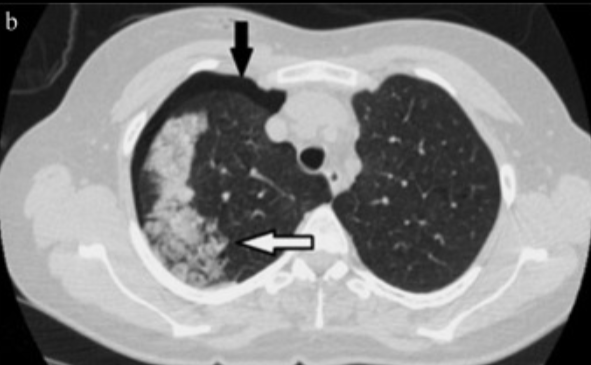
\includegraphics[width=0.7\textwidth]{img/complicacion.png}
    \caption{Neumotórax y hemorragia alveolar grado 2 como complicaciones tras la realización de una biopsia pulmonar guiada por TC \parencite{elshafee2019complications}.}
    \label{fig:complicaciones}
\end{figure}

Como se ha mencionado, hay numerosos estudios que aportan evidencia sobre la determinación de la benignidad o malignidad de distintos nódulos pulmonares, así como sobre la clasificación de diferentes tipos de neoplasias. Sin embargo, son escasos los trabajos que abordan el análisis de la probabilidad de desarrollar una complicación antes de realizar una biopsia.

Por ello, desarrollar modelos capaces de predecir el riesgo de complicaciones antes de la biopsia resulta especialmente relevante, ya que permitiría optimizar recursos médicos, planificar medidas preventivas y reducir la incidencia de eventos adversos.



\section{Propuesta}

Este trabajo propone el desarrollo de un sistema predictivo basado en técnicas de aprendizaje profundo y radiómica para anticipar el riesgo de complicaciones asociadas a biopsias pulmonares guiadas por TC. La idea central es construir un modelo capaz de analizar imágenes médicas tridimensionales junto con datos clínicos tabulares para estimar la probabilidad de complicaciones antes del procedimiento.

Para ello, se plantea integrar enfoques de radiómica y Deep Learning, que han demostrado un gran potencial en el análisis de imágenes médicas al facilitar la extracción automática de patrones complejos y mejorar la capacidad predictiva de los modelos \parencite{shen2017deep}. La radiómica ofrece un marco para extraer información cuantitativa de las imágenes, combinando características semánticas evaluadas por radiólogos con descriptores generados automáticamente. Este proceso requiere un flujo de trabajo estructurado que incluye la adquisición de las imágenes, la segmentación de las regiones de interés, la extracción de características y la construcción del modelo predictivo. Las Figuras~\ref{fig:compcaracteristicas_radiomica-label} y~\ref{fig:radiomica2-label} ilustran tanto la evolución de los tipos de características extraídas como el esquema general del flujo de trabajo que combina canales de radiómica convencional y aprendizaje profundo.

\begin{figure}[!htbp]
    \centering
    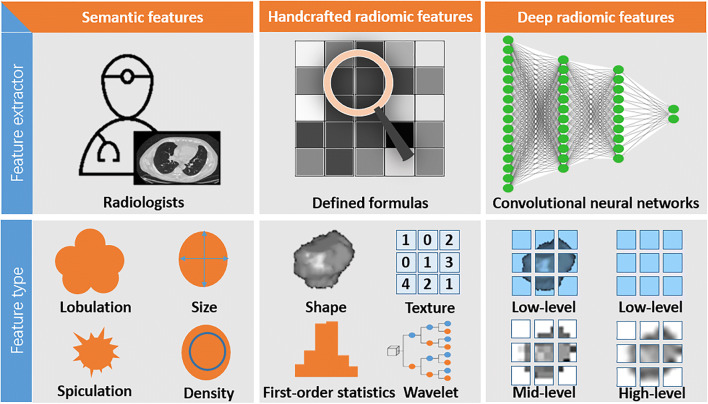
\includegraphics[width=0.9\textwidth]{img/comp_radiomica.jpg}
    \caption{Comparación de características semánticas, radiómicas manuales y radiómicas profundas \parencite{wu2021structural}.}
    \label{fig:compcaracteristicas_radiomica-label}
\end{figure}

\begin{figure}[!htbp]
    \centering
    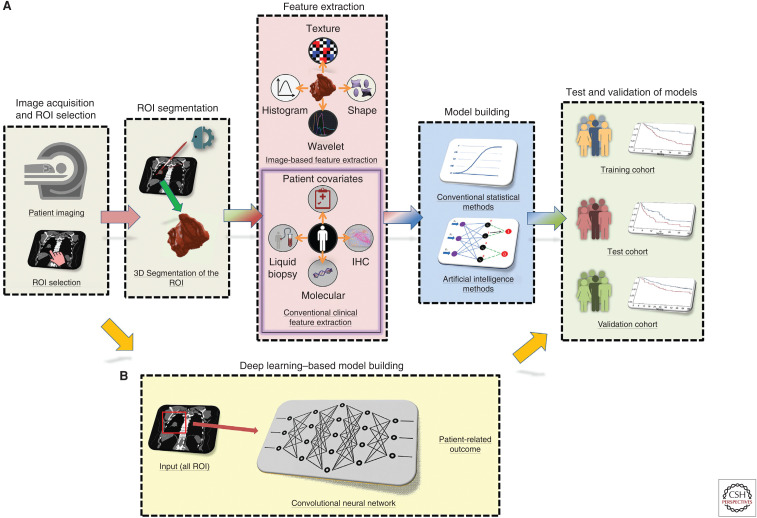
\includegraphics[width=1\textwidth]{img/radiomica2.jpg}
    \caption{Procesos de modelado de biomarcadores basados en imágenes. (A) Canal de radiómica convencional. (B) Canal de aprendizaje profundo. (ROI) Región de interés, (IHC) inmunohistoquímica \parencite{leiter2023global}.}
    \label{fig:radiomica2-label}
\end{figure}


Dada la ausencia de literatura previa en este campo concreto, la propuesta representa una línea de investigación novedosa. No existen modelos ni estrategias validadas para abordar la predicción del riesgo de complicaciones en biopsias pulmonares con inteligencia artificial (IA). Por ello, el diseño del presente estudio incluyó fases exploratorias para evaluar la viabilidad del enfoque, identificar limitaciones técnicas y comparar múltiples estrategias de modelado.

\section{Estructura del trabajo}
El contenido del trabajo se divide en dos partes:

\subsection*{Parte I: Matemáticas}

La primera parte proporciona el marco teórico y fundamento matemático necesario para entender las técnicas utilizadas en el la segunda parte. Comienza con la teoría de procesamiento de señales (Capítulo \ref{chap:señales}), donde se introducen conceptos fundamentales como la definición de señal, las transformadas de Fourier, la operación de convolución y la radiómica. A continuación, en  el Capítulo \ref{chap:optimizacion}, se abordan métodos de optimización basados en gradientes y optimización convexa, necesarios para garantizar la convergencia de los modelos.

En los fundamentos matemáticos del aprendizaje automático (Capítulo \ref{chap:aa-mates}), se detallan los tipos de aprendizaje (supervisado y no supervisado), centrándonos en el problema de clasificación. El aprendizaje profundo (Capítulo \ref{chap:dl-mates}) cubre la propagación hacia adelante, el algoritmo de backpropagation, las funciones de coste, las unidades de activación, el aprendizaje por transferencia y las redes neuronales convolucionales. Finalmente, los fundamentos métricos para el procesamiento avanzado de datos (Capítulo \ref{chap:metric-learning-mates}) profundizan en el aprendizaje de métricas de distancia, tanto en sus formulaciones lineales como no lineales.

\subsection*{Parte II: Informática}

La segunda parte aplica los conceptos teóricos para construir de forma práctica el sistema predictivo. Se inicia con el planteamiento del problema (Capítulo \ref{chap:planteamiento-problema}), donde se describe el contexto clínico, la motivación médica y las dificultades inherentes a la predicción de complicaciones en biopsias pulmonares. En el análisis de datos y preprocesamiento (Capítulo \ref{eda}), se detallan la adquisición, exploración y preparación de volúmenes TC mediante segmentación pulmonar, así como la normalización de datos clínicos tabulares.

El modelado con deep learning (Capítulo \ref{chap:dl-info}) incluye el desarrollo de arquitecturas 2D y 3D, estrategias avanzadas como el preentrenamiento, el fine-tuning y el aprendizaje contrastivo, además de la integración de datos clínicos e imágenes en modelos multimodales. En el análisis radiómico y machine learning clásico (Capítulo \ref{chap:aa-radiomica}) se abordan la extracción y el análisis de características radiómicas mediante técnicas de aprendizaje automático tradicional. El análisis experimental (Capítulo \ref{analisis-resultados}) describe la validación cruzada estratificada, el diseño de experimentos y el análisis detallado de resultados con métricas estándar. Finalmente, en el Capítulo \ref{chap:explicabilidad} se analizan los resultados con técnicas de explicabilidad, incluyendo métodos como Grad-CAM y SHAP, así como el análisis radiómico orientado a facilitar la interpretación y validación clínica de las predicciones.


\section{Objetivos}
Los objetivos inicialmente previstos en la propuesta del TFG fueron divididos en dos partes. 

En la parte de Matemáticas se persigue como objetivo fundamental proporcionar el soporte teórico necesario para entender las técnicas empleadas en el procesamiento y análisis de imágenes médicas. Para ello, se plantean los siguientes objetivos:

\begin{itemize}
    \item Estudiar los conceptos de señal, procesamiento de señales y teoría de radiómica.
    \item Comprender la teoría de optimización, incluyendo métodos basados en gradientes y propiedades de la convexidad.
    \item Analizar los fundamentos del aprendizaje automático y profundo, desde los principios básicos de clasificación hasta el funcionamiento de redes neuronales.
\end{itemize}


En la parte de Informática tiene como objetivo aplicar estos fundamentos para desarrollar de forma práctica el sistema predictivo. En este bloque se proponen los siguientes objetivos específicos:

\begin{itemize}
    \item Analizar y preprocesar datos clínicos tabulares y volúmenes de TC, incluyendo segmentación pulmonar, normalización y homogenización de datos para su uso en modelos.
    \item Desarrollar estrategias de modelado basadas en redes neuronales convolucionales 2D y 3D, definiendo arquitecturas, procedimientos de entrenamiento y estrategias avanzadas como el preentrenamiento y fine-tuning.
    \item Integrar datos clínicos con imágenes médicas para construir modelos multimodales capaces de aprovechar toda la información disponible.
    \item Aplicar técnicas de radiómica para extraer características relevantes de las imágenes y emplearlas en modelos clásicos de aprendizaje automático.
    \item Diseñar una experimentación adecuada que incluya validación cruzada estratificada para evaluar de manera robusta el rendimiento del sistema, mitigando problemas derivados del tamaño reducido de la muestra.
    \item Realizar un análisis detallado de los resultados, incorporando métricas estándar de evaluación y aplicando técnicas de explicabilidad para interpretar las predicciones y facilitar su validación clínica.
\end{itemize}


Finalmente, cabe señalar que los objetivos planteados se han cumplido en términos generales, logrando desarrollar un sistema predictivo funcional que integra las distintas etapas de procesamiento de datos, modelado y análisis. Sin embargo, los resultados obtenidos todavía muestran margen de mejora por varias razones. A lo largo del proyecto, la disponibilidad de datos fue aumentando de forma progresiva, lo que obligó a replantear y ajustar los experimentos en diferentes fases. Además, el conjunto inicial presentaba un fuerte desbalanceo entre clases que requirió técnicas específicas para mitigarlo. En general, el tamaño limitado del conjunto de datos redujo la capacidad de generalización de los modelos. Por último, el trabajo se llevó a cabo sin contar con una base de literatura consolidada específica para este problema clínico, lo que implicó diseñar soluciones desde cero y adaptar estrategias de problemas similares.



\section{Bibliografía fundamental}
A lo largo del trabajo se han consultado numerosas fuentes, pero entre ellas se puede destacar la siguiente bibliografía:

\begin{itemize}
    \item Goodfellow, I., Bengio, Y., Courville, A. y Bengio, Y. (2016). \textit{Deep learning} (Vol. 1, No. 2). Cambridge: MIT Press. Utilizada para el estudio de la teoría de optimización y los fundamentos de Deep Learning. 
    \item Shalev-Shwartz, S., y Ben-David, S. (2014). \textit{Understanding machine learning: From theory to algorithms}. Cambridge University Press. Utilizada para los fundamentos de aprendizaje automático y fundamentos del aprendizaje de métricas de distancias.
    \item Un artículo fundamental para el estudio de la radiómica y su base matemática: de Vaucleroy, N., Macq, B., De Vleeschouwer, C., y Léger, J. \textit{Mathematical morphology applied to Radiomics}.
    \item Artículos relacionados con la parte práctica aplicada a medicina: \cite{shur2021radiomics}, \cite{mukherjee2022radiomics}, \cite{suara2023grad}, \cite{calzado2010tomografia} y \cite{shen2017deep}. 
\end{itemize}



\endinput
